\documentclass[twoside]{book}

% Packages required by doxygen
\usepackage{fixltx2e}
\usepackage{calc}
\usepackage{doxygen}
\usepackage[export]{adjustbox} % also loads graphicx
\usepackage{graphicx}
\usepackage[utf8]{inputenc}
\usepackage{makeidx}
\usepackage{multicol}
\usepackage{multirow}
\PassOptionsToPackage{warn}{textcomp}
\usepackage{textcomp}
\usepackage[nointegrals]{wasysym}
\usepackage[table]{xcolor}

% Font selection
\usepackage[T1]{fontenc}
\usepackage[scaled=.90]{helvet}
\usepackage{courier}
\usepackage{amssymb}
\usepackage{sectsty}
\renewcommand{\familydefault}{\sfdefault}
\allsectionsfont{%
  \fontseries{bc}\selectfont%
  \color{darkgray}%
}
\renewcommand{\DoxyLabelFont}{%
  \fontseries{bc}\selectfont%
  \color{darkgray}%
}
\newcommand{\+}{\discretionary{\mbox{\scriptsize$\hookleftarrow$}}{}{}}

% Page & text layout
\usepackage{geometry}
\geometry{%
  a4paper,%
  top=2.5cm,%
  bottom=2.5cm,%
  left=2.5cm,%
  right=2.5cm%
}
\tolerance=750
\hfuzz=15pt
\hbadness=750
\setlength{\emergencystretch}{15pt}
\setlength{\parindent}{0cm}
\setlength{\parskip}{3ex plus 2ex minus 2ex}
\makeatletter
\renewcommand{\paragraph}{%
  \@startsection{paragraph}{4}{0ex}{-1.0ex}{1.0ex}{%
    \normalfont\normalsize\bfseries\SS@parafont%
  }%
}
\renewcommand{\subparagraph}{%
  \@startsection{subparagraph}{5}{0ex}{-1.0ex}{1.0ex}{%
    \normalfont\normalsize\bfseries\SS@subparafont%
  }%
}
\makeatother

% Headers & footers
\usepackage{fancyhdr}
\pagestyle{fancyplain}
\fancyhead[LE]{\fancyplain{}{\bfseries\thepage}}
\fancyhead[CE]{\fancyplain{}{}}
\fancyhead[RE]{\fancyplain{}{\bfseries\leftmark}}
\fancyhead[LO]{\fancyplain{}{\bfseries\rightmark}}
\fancyhead[CO]{\fancyplain{}{}}
\fancyhead[RO]{\fancyplain{}{\bfseries\thepage}}
\fancyfoot[LE]{\fancyplain{}{}}
\fancyfoot[CE]{\fancyplain{}{}}
\fancyfoot[RE]{\fancyplain{}{\bfseries\scriptsize Generated by Doxygen }}
\fancyfoot[LO]{\fancyplain{}{\bfseries\scriptsize Generated by Doxygen }}
\fancyfoot[CO]{\fancyplain{}{}}
\fancyfoot[RO]{\fancyplain{}{}}
\renewcommand{\footrulewidth}{0.4pt}
\renewcommand{\chaptermark}[1]{%
  \markboth{#1}{}%
}
\renewcommand{\sectionmark}[1]{%
  \markright{\thesection\ #1}%
}

% Indices & bibliography
\usepackage{natbib}
\usepackage[titles]{tocloft}
\setcounter{tocdepth}{3}
\setcounter{secnumdepth}{5}
\makeindex

% Hyperlinks (required, but should be loaded last)
\usepackage{ifpdf}
\ifpdf
  \usepackage[pdftex,pagebackref=true]{hyperref}
\else
  \usepackage[ps2pdf,pagebackref=true]{hyperref}
\fi
\hypersetup{%
  colorlinks=true,%
  linkcolor=blue,%
  citecolor=blue,%
  unicode%
}

% Custom commands
\newcommand{\clearemptydoublepage}{%
  \newpage{\pagestyle{empty}\cleardoublepage}%
}

\usepackage{caption}
\captionsetup{labelsep=space,justification=centering,font={bf},singlelinecheck=off,skip=4pt,position=top}

%===== C O N T E N T S =====

\begin{document}

% Titlepage & ToC
\hypersetup{pageanchor=false,
             bookmarksnumbered=true,
             pdfencoding=unicode
            }
\pagenumbering{alph}
\begin{titlepage}
\vspace*{7cm}
\begin{center}%
{\Large Algo\+\_\+\+Galaxy \\[1ex]\large 0.\+1 }\\
\vspace*{1cm}
{\large Generated by Doxygen 1.8.13}\\
\end{center}
\end{titlepage}
\clearemptydoublepage
\pagenumbering{roman}
\tableofcontents
\clearemptydoublepage
\pagenumbering{arabic}
\hypersetup{pageanchor=true}

%--- Begin generated contents ---
\chapter{Data Structure Index}
\section{Data Structures}
Here are the data structures with brief descriptions\+:\begin{DoxyCompactList}
\item\contentsline{section}{\hyperlink{struct__body}{\+\_\+body} }{\pageref{struct__body}}{}
\item\contentsline{section}{\hyperlink{struct_body}{Body} \\*Physic body with a position, a velocity and a mass }{\pageref{struct_body}}{}
\end{DoxyCompactList}

\chapter{File Index}
\section{File List}
Here is a list of all documented files with brief descriptions\+:\begin{DoxyCompactList}
\item\contentsline{section}{headers/\hyperlink{two__bodies_8h}{two\+\_\+bodies.\+h} \\*Struct and function prototypes of \hyperlink{two__bodies_8c_source}{two\+\_\+bodies.\+c} }{\pageref{two__bodies_8h}}{}
\item\contentsline{section}{src/{\bfseries two\+\_\+bodies.\+c} }{\pageref{two__bodies_8c}}{}
\end{DoxyCompactList}

\chapter{Data Structure Documentation}
\hypertarget{struct__body}{}\section{\+\_\+body Struct Reference}
\label{struct__body}\index{\+\_\+body@{\+\_\+body}}
\subsection*{Data Fields}
\begin{DoxyCompactItemize}
\item 
double \hyperlink{struct__body_a9c1e50fd3234caf28c5f65a912b5c16a}{px}
\item 
double \hyperlink{struct__body_ad29ba68eddcdfabc5dd4e8e213a0f5cd}{py}
\item 
double \hyperlink{struct__body_a2d31cc80a747457c212675a58c68b2b1}{vx}
\item 
double \hyperlink{struct__body_a42e75115788e629a258d041808d822a0}{vy}
\item 
double \hyperlink{struct__body_aa7e88347476ef454086e7c3cd9865460}{fx}
\item 
double \hyperlink{struct__body_a03c4ce20c7e4b8c6d60a20b833be69fe}{fy}
\item 
double \hyperlink{struct__body_a244bf42c46054cf1113be44d55f2156d}{mass}
\end{DoxyCompactItemize}


\subsection{Detailed Description}


Definition at line 23 of file two\+\_\+bodies.\+h.



\subsection{Field Documentation}
\mbox{\Hypertarget{struct__body_aa7e88347476ef454086e7c3cd9865460}\label{struct__body_aa7e88347476ef454086e7c3cd9865460}} 
\index{\+\_\+body@{\+\_\+body}!fx@{fx}}
\index{fx@{fx}!\+\_\+body@{\+\_\+body}}
\subsubsection{\texorpdfstring{fx}{fx}}
{\footnotesize\ttfamily double fx}

x force 

Definition at line 29 of file two\+\_\+bodies.\+h.

\mbox{\Hypertarget{struct__body_a03c4ce20c7e4b8c6d60a20b833be69fe}\label{struct__body_a03c4ce20c7e4b8c6d60a20b833be69fe}} 
\index{\+\_\+body@{\+\_\+body}!fy@{fy}}
\index{fy@{fy}!\+\_\+body@{\+\_\+body}}
\subsubsection{\texorpdfstring{fy}{fy}}
{\footnotesize\ttfamily double fy}

y force 

Definition at line 30 of file two\+\_\+bodies.\+h.

\mbox{\Hypertarget{struct__body_a244bf42c46054cf1113be44d55f2156d}\label{struct__body_a244bf42c46054cf1113be44d55f2156d}} 
\index{\+\_\+body@{\+\_\+body}!mass@{mass}}
\index{mass@{mass}!\+\_\+body@{\+\_\+body}}
\subsubsection{\texorpdfstring{mass}{mass}}
{\footnotesize\ttfamily double mass}

mass 

Definition at line 31 of file two\+\_\+bodies.\+h.

\mbox{\Hypertarget{struct__body_a9c1e50fd3234caf28c5f65a912b5c16a}\label{struct__body_a9c1e50fd3234caf28c5f65a912b5c16a}} 
\index{\+\_\+body@{\+\_\+body}!px@{px}}
\index{px@{px}!\+\_\+body@{\+\_\+body}}
\subsubsection{\texorpdfstring{px}{px}}
{\footnotesize\ttfamily double px}

x position 

Definition at line 25 of file two\+\_\+bodies.\+h.

\mbox{\Hypertarget{struct__body_ad29ba68eddcdfabc5dd4e8e213a0f5cd}\label{struct__body_ad29ba68eddcdfabc5dd4e8e213a0f5cd}} 
\index{\+\_\+body@{\+\_\+body}!py@{py}}
\index{py@{py}!\+\_\+body@{\+\_\+body}}
\subsubsection{\texorpdfstring{py}{py}}
{\footnotesize\ttfamily double py}

y position 

Definition at line 26 of file two\+\_\+bodies.\+h.

\mbox{\Hypertarget{struct__body_a2d31cc80a747457c212675a58c68b2b1}\label{struct__body_a2d31cc80a747457c212675a58c68b2b1}} 
\index{\+\_\+body@{\+\_\+body}!vx@{vx}}
\index{vx@{vx}!\+\_\+body@{\+\_\+body}}
\subsubsection{\texorpdfstring{vx}{vx}}
{\footnotesize\ttfamily double vx}

x velocity 

Definition at line 27 of file two\+\_\+bodies.\+h.

\mbox{\Hypertarget{struct__body_a42e75115788e629a258d041808d822a0}\label{struct__body_a42e75115788e629a258d041808d822a0}} 
\index{\+\_\+body@{\+\_\+body}!vy@{vy}}
\index{vy@{vy}!\+\_\+body@{\+\_\+body}}
\subsubsection{\texorpdfstring{vy}{vy}}
{\footnotesize\ttfamily double vy}

y velocity 

Definition at line 28 of file two\+\_\+bodies.\+h.



The documentation for this struct was generated from the following file\+:\begin{DoxyCompactItemize}
\item 
headers/\hyperlink{two__bodies_8h}{two\+\_\+bodies.\+h}\end{DoxyCompactItemize}

\hypertarget{struct_body}{}\section{Body Struct Reference}
\label{struct_body}\index{Body@{Body}}


Physic body with a position, a velocity and a mass.  




{\ttfamily \#include $<$two\+\_\+bodies.\+h$>$}



\subsection{Detailed Description}
Physic body with a position, a velocity and a mass. 

This is a body to simulate physics. 

The documentation for this struct was generated from the following file\+:\begin{DoxyCompactItemize}
\item 
headers/\hyperlink{two__bodies_8h}{two\+\_\+bodies.\+h}\end{DoxyCompactItemize}

\chapter{File Documentation}
\hypertarget{two__bodies_8h}{}\section{headers/two\+\_\+bodies.h File Reference}
\label{two__bodies_8h}\index{headers/two\+\_\+bodies.\+h@{headers/two\+\_\+bodies.\+h}}


Struct and function prototypes of \hyperlink{two__bodies_8c_source}{two\+\_\+bodies.\+c}.  


This graph shows which files directly or indirectly include this file\+:
\nopagebreak
\begin{figure}[H]
\begin{center}
\leavevmode
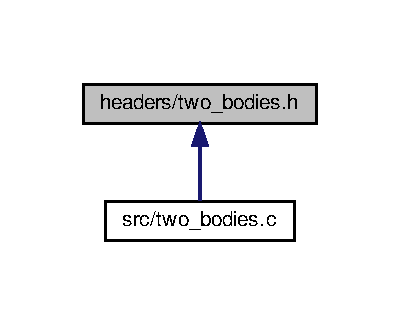
\includegraphics[width=192pt]{two__bodies_8h__dep__incl}
\end{center}
\end{figure}
\subsection*{Data Structures}
\begin{DoxyCompactItemize}
\item 
struct \hyperlink{struct__body}{\+\_\+body}
\end{DoxyCompactItemize}
\subsection*{Macros}
\begin{DoxyCompactItemize}
\item 
\mbox{\Hypertarget{two__bodies_8h_a498d9f026138406895e9a34b504ac6a6}\label{two__bodies_8h_a498d9f026138406895e9a34b504ac6a6}} 
\#define {\bfseries W\+I\+N\+D\+O\+W\+\_\+\+W\+I\+D\+TH}~400
\item 
\mbox{\Hypertarget{two__bodies_8h_a5473cf64fa979b48335079c99532e243}\label{two__bodies_8h_a5473cf64fa979b48335079c99532e243}} 
\#define {\bfseries W\+I\+N\+D\+O\+W\+\_\+\+H\+E\+I\+G\+HT}~400
\item 
\mbox{\Hypertarget{two__bodies_8h_a355d118391f55e89a4c7ba380d40b83a}\label{two__bodies_8h_a355d118391f55e89a4c7ba380d40b83a}} 
\#define {\bfseries W\+I\+D\+T\+H\+\_\+\+O\+F\+\_\+\+R\+E\+G\+I\+ON}~4e4
\item 
\#define \hyperlink{two__bodies_8h_aed9ea78689ecce0b7264c02c7f8a9a54}{G}~6.\+674e-\/11
\item 
\#define \hyperlink{two__bodies_8h_a84d2e204243c4a836de9b0a8ead3d376}{dt}~0.\+1
\end{DoxyCompactItemize}
\subsection*{Typedefs}
\begin{DoxyCompactItemize}
\item 
\mbox{\Hypertarget{two__bodies_8h_a3f72d8996ae0946a2480f0693fd3d107}\label{two__bodies_8h_a3f72d8996ae0946a2480f0693fd3d107}} 
typedef struct \hyperlink{struct__body}{\+\_\+body} {\bfseries Body}
\end{DoxyCompactItemize}
\subsection*{Functions}
\begin{DoxyCompactItemize}
\item 
\mbox{\Hypertarget{two__bodies_8h_a499e668b74b978e5872912c9f01e9c21}\label{two__bodies_8h_a499e668b74b978e5872912c9f01e9c21}} 
void {\bfseries draw\+\_\+body} (\hyperlink{struct_body}{Body} $\ast$B)
\end{DoxyCompactItemize}


\subsection{Detailed Description}
Struct and function prototypes of \hyperlink{two__bodies_8c_source}{two\+\_\+bodies.\+c}. 

\begin{DoxyAuthor}{Author}
Marti Emilie \& Soustre Ludovic 
\end{DoxyAuthor}
\begin{DoxyVersion}{Version}
0.\+1 
\end{DoxyVersion}


\subsection{Macro Definition Documentation}
\mbox{\Hypertarget{two__bodies_8h_a84d2e204243c4a836de9b0a8ead3d376}\label{two__bodies_8h_a84d2e204243c4a836de9b0a8ead3d376}} 
\index{two\+\_\+bodies.\+h@{two\+\_\+bodies.\+h}!dt@{dt}}
\index{dt@{dt}!two\+\_\+bodies.\+h@{two\+\_\+bodies.\+h}}
\subsubsection{\texorpdfstring{dt}{dt}}
{\footnotesize\ttfamily \#define dt~0.\+1}

time step 

Definition at line 15 of file two\+\_\+bodies.\+h.

\mbox{\Hypertarget{two__bodies_8h_aed9ea78689ecce0b7264c02c7f8a9a54}\label{two__bodies_8h_aed9ea78689ecce0b7264c02c7f8a9a54}} 
\index{two\+\_\+bodies.\+h@{two\+\_\+bodies.\+h}!G@{G}}
\index{G@{G}!two\+\_\+bodies.\+h@{two\+\_\+bodies.\+h}}
\subsubsection{\texorpdfstring{G}{G}}
{\footnotesize\ttfamily \#define G~6.\+674e-\/11}

the gravitational constant 

Definition at line 14 of file two\+\_\+bodies.\+h.


%--- End generated contents ---

% Index
\backmatter
\newpage
\phantomsection
\clearemptydoublepage
\addcontentsline{toc}{chapter}{Index}
\printindex

\end{document}
